\section{API-Werkzeuge}
\label{sec:api-tools}

Der Literaturüberblick sollte nicht nur einen Eindruck über den Forschungsstand vermitteln, sondern auch die Einsicht erleichtern, dass nicht alle API-Usability-Probleme in dem \gls{api} selbst gelöst werden können.

Dieser Abschnitt befasst sich mit konkreten Lösungsansätzen, die nicht bei der API selbst, sondern bei den übrigen Einflussfaktoren, wie der Dokumentation, ansetzen. In Anbetracht des Umfangs dieser Literaturübersicht und der Vielzahl existierender Werkzeuge, beschränke ich mich auf eine sehr knappe Beschreibung letzterer.

Ein Vergleich der hier vorgestellten Werkzeuge ist knifflig, da sich auch augenscheinlich ähnliche Werkzeuge im Detail stark unterscheiden. Ich habe mich entschlossen, die Werkzeuge nach ihrer Zielgruppe\footnote{Nicht zu verwechseln mit der schlussendlich profitierenden Gruppe, die immer aus API-Anwendern und API-Endanwendern besteht.} zu gruppieren und nach dem Aufwand für die API-Entwickler zu sortieren. \fref{fig:api-tools} ordnet die Werkzeuge entlang dieser beiden Dimensionen ein und zeigt durch den grafischen Marker, welches primäre Ziel von den Werkzeugen verfolgt wird. Diese Einordnung spiegelt meine persönliche Einschätzung wider und ist im besten Falle unscharf\footnote{Insbesondere Werkzeuge, die sich nach meiner Einschätzung für API-Endanwender eignen, wurden von den Autoren in den meisten Fällen nie unter diesem Gesichtspunkt entwickelt. Der Begriff der Zielgruppe trifft also nicht ganz zu.}.

\newgeometry{inner=2cm,outer=1.5cm,top=1.5cm,bottom=1.5cm}
\thispagestyle{empty}
\begin{landscape}
\begin{figure}
  \centering
    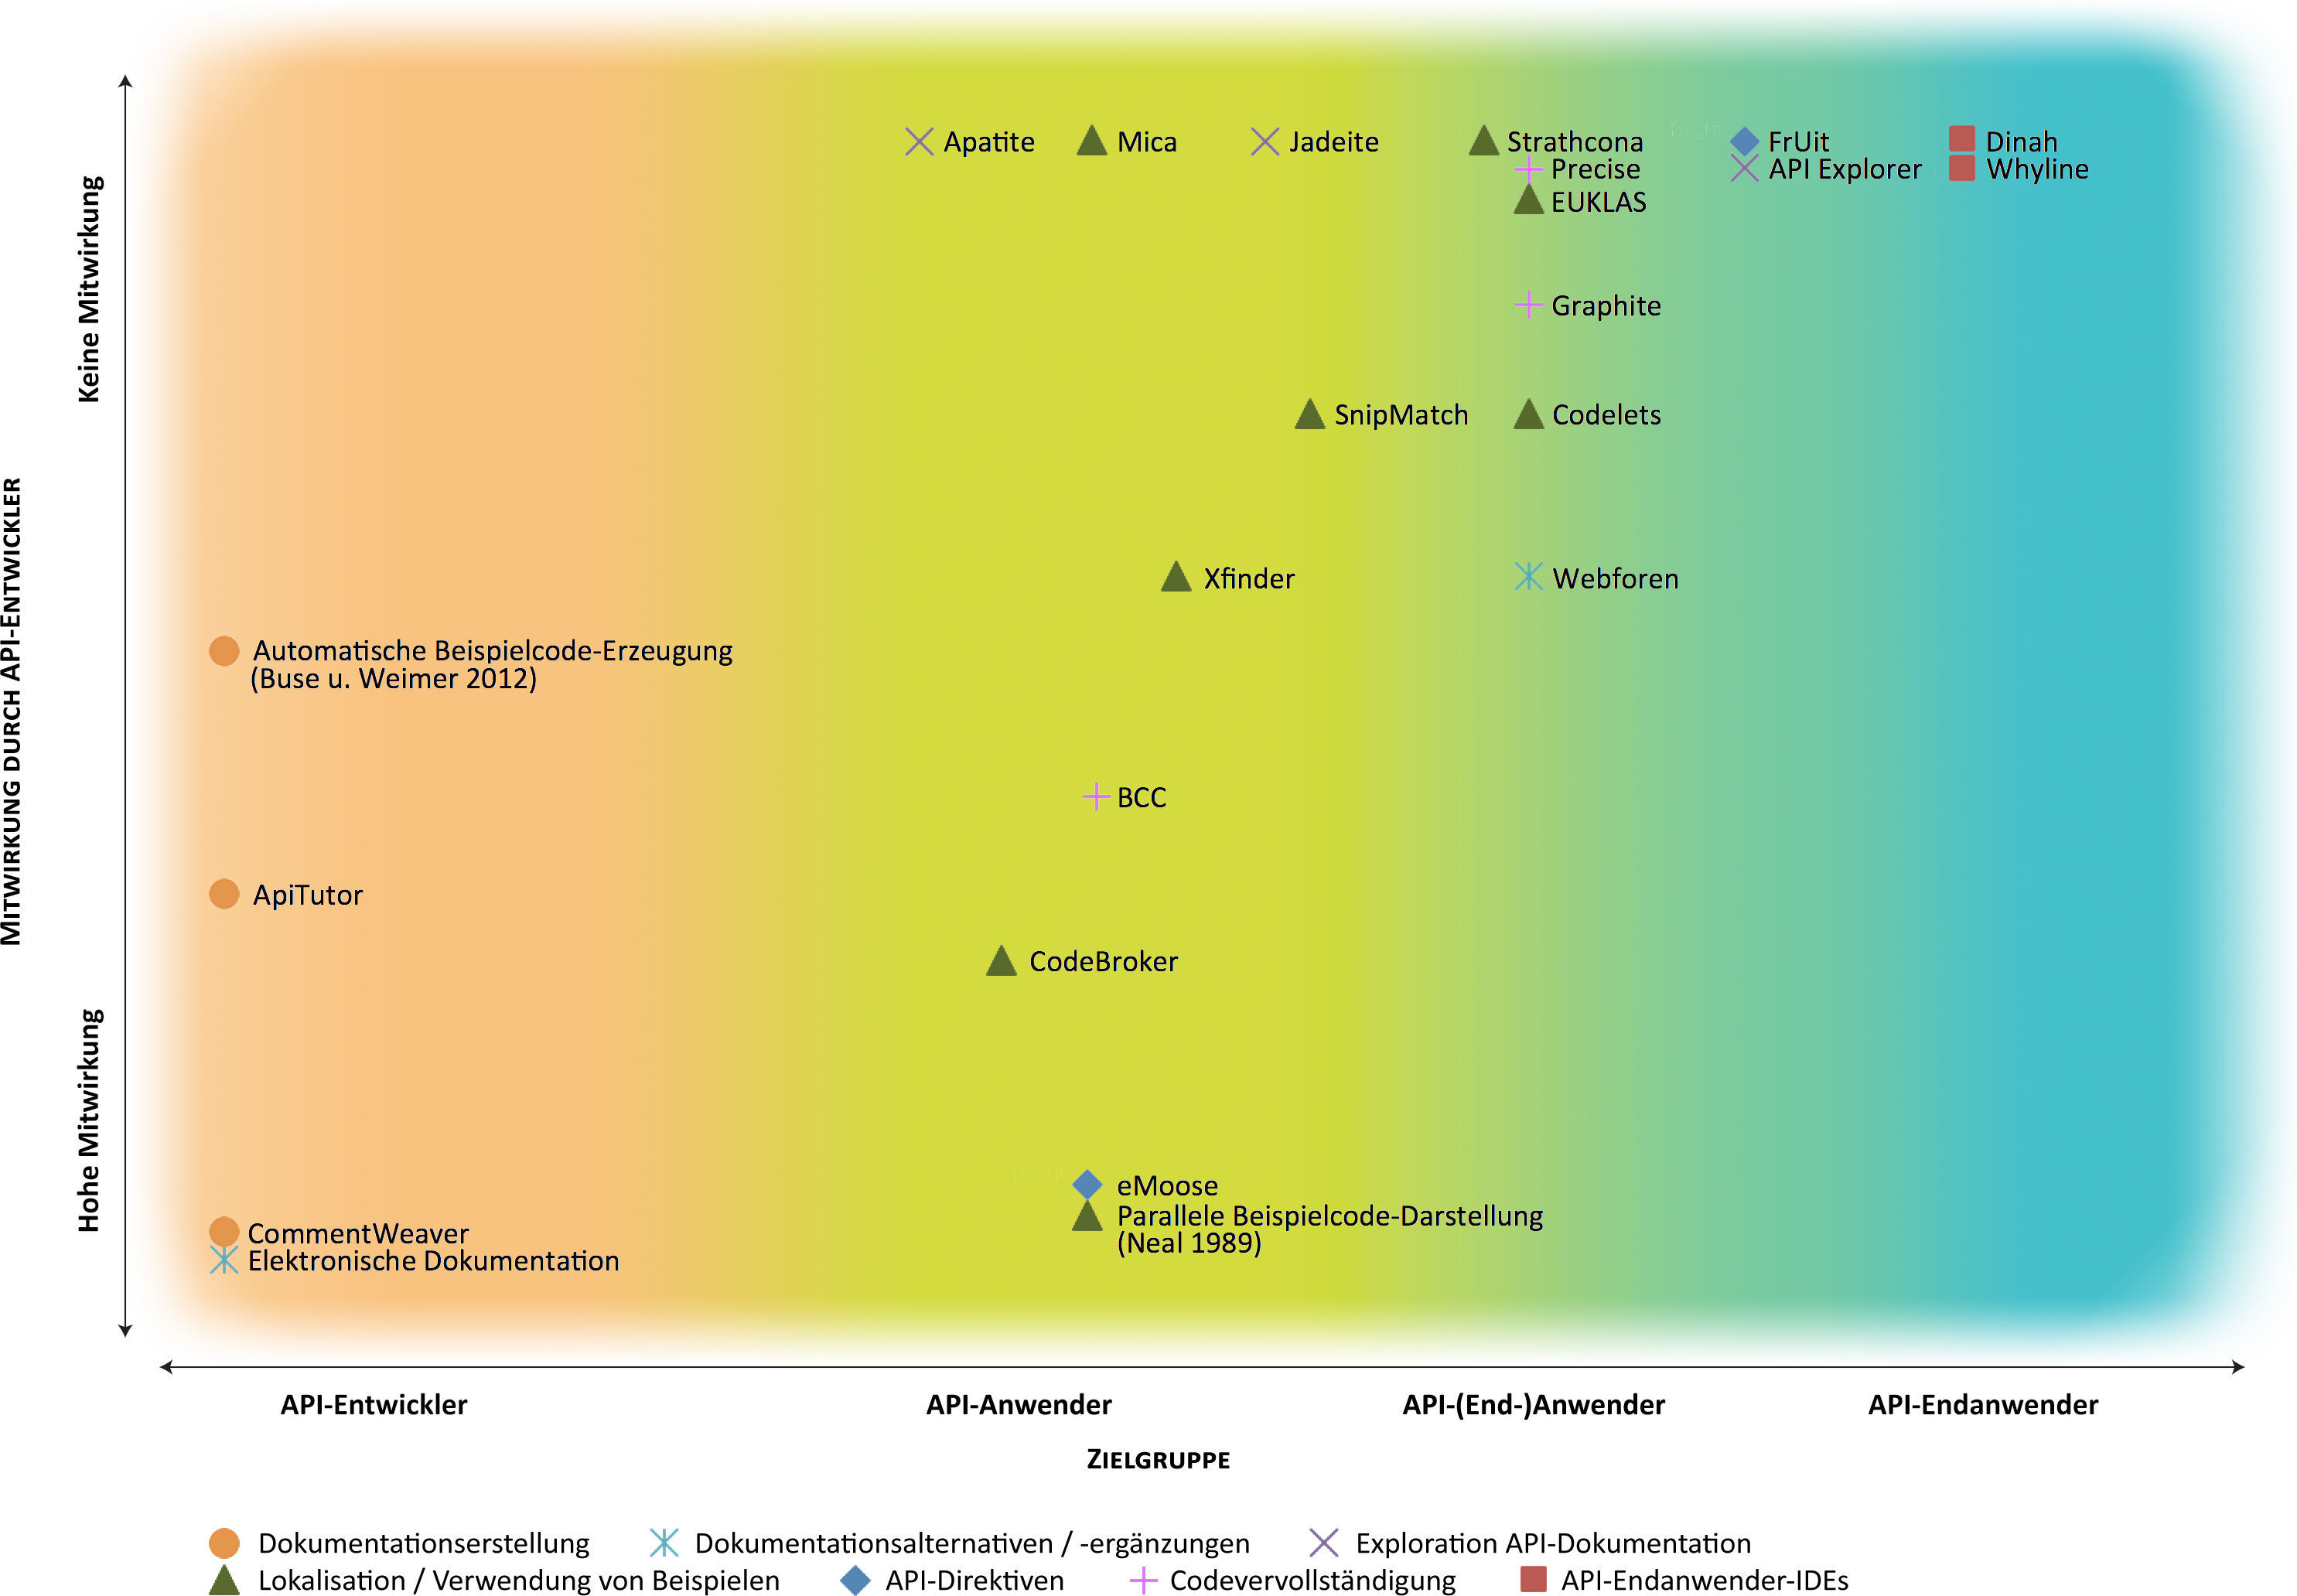
\includegraphics[width=0.87\linewidth]{Figures/tools/api-tools.png}
  \caption[Einteilung von API-Werkzeugen]{Grobe Einordnung von API-Werkzeugen entlang der Dimensionen \textit{Zielgruppe} und \textit{Mitwirkung durch API-Entwickler}. Die Ikone stellt dar, welches primäre Ziel vom jeweiligen Werkzeug verfolgt wird.}
  \label{fig:api-tools}
\end{figure}
\end{landscape}
\restoregeometry





\subsection{Werkzeuge für API-Entwickler}

\textit{CommentWeaver} \citep{Horie:2010dq} ist eine JavaDoc-Erweiterung, die API-Entwickler bei der Erstellung von API-Dokumentationen unterstützt. Das Werkzeug löst das Problem von verteilt dokumentierten API-Aspekten, indem es verschiedene Mechanismen anbietet, die die modulare Dokumentation einer API erlaubt. Beispielsweise können Dokumentationseinheiten annotiert werden, womit definiert wird, an welcher Stelle dieser Eintrag in der Dokumentation erscheint.

\textit{ApiTutor} \citep{Dahotre:2011vr} ist ein Werkzeug, das API-Entwickler dabei unterstützen soll, Tutorials für API-Anwender zu entwickeln. In meinen Augen ist der Nutzen allerdings nicht höher als der Aufwand für die API-Entwickler\footnote{Der Ablauf besteht in einer integrierten Suchmaschinen-Abfrage und der anschließenden Auswahl von Code-Beispielen, die dann schließlich vom Tutorial-Verfasser didaktisch aufgearbeitet werden.}, was durch die ausbleibende Beachtung dieser Arbeit bestätigt wird.

\begin{important}
\cite{Buse:2012vv} stellen in ihrer Arbeit einen Algorithmus, der in der Lage ist, mit Hilfe von API-Anwendungscode automatisch menschenlesbare Code-Beispiele für die verschiedenen API-Elemente zu erzeugen (siehe Listung \ref{lst:auto-code-example}). Die Forscher konnten mit einer 154 Probanden umfassenden Studie an Hand von 35 Standard-Java-Klassen zeigen, dass 82\% der generierten Beispiele als mindestens gleich gut eingeschätzt wurden, wie von Menschen geschriebene Beispiele.
\end{important}

\begin{center}
\begin{minted}[linenos, firstnumber=1, autogobble=false]{xml}
FileReader f; //initialized previously
BufferedReader br = new BufferedReader(f);
while(br.ready()) {
String line = br.readLine();
   //do something with line
}
br.close();
\end{minted}
\captionof{listing}{Automatisch generiertes Code-Beispiel \cite{Buse:2012vv}}
\label{lst:auto-code-example}
\end{center}



\subsection{Werkzeuge für API-Anwender}

Eine sehr frühe Arbeit auf diesem Gebiet stammt von \cite{Neal:1989ef}. Sie prägten den Begriff der Beispiel-basierten Programmierung (engl. \textit{example-based programming}), den ich als Teilgebiet der Anwendungswiederverwendung verstehe. Dazu wurde ein existierender Codeeditor um die Funktion erweitert, neben dem bereits vorhandenen Editorbereich einen zweiten neuen Bereich mit Anwendungsbeispielen darzustellen (siehe \fref{fig:neal}). Die Beispiele müssen zuvor allerdings manuell erstellt werden.

\begin{figure}[!ht]
  \centering
    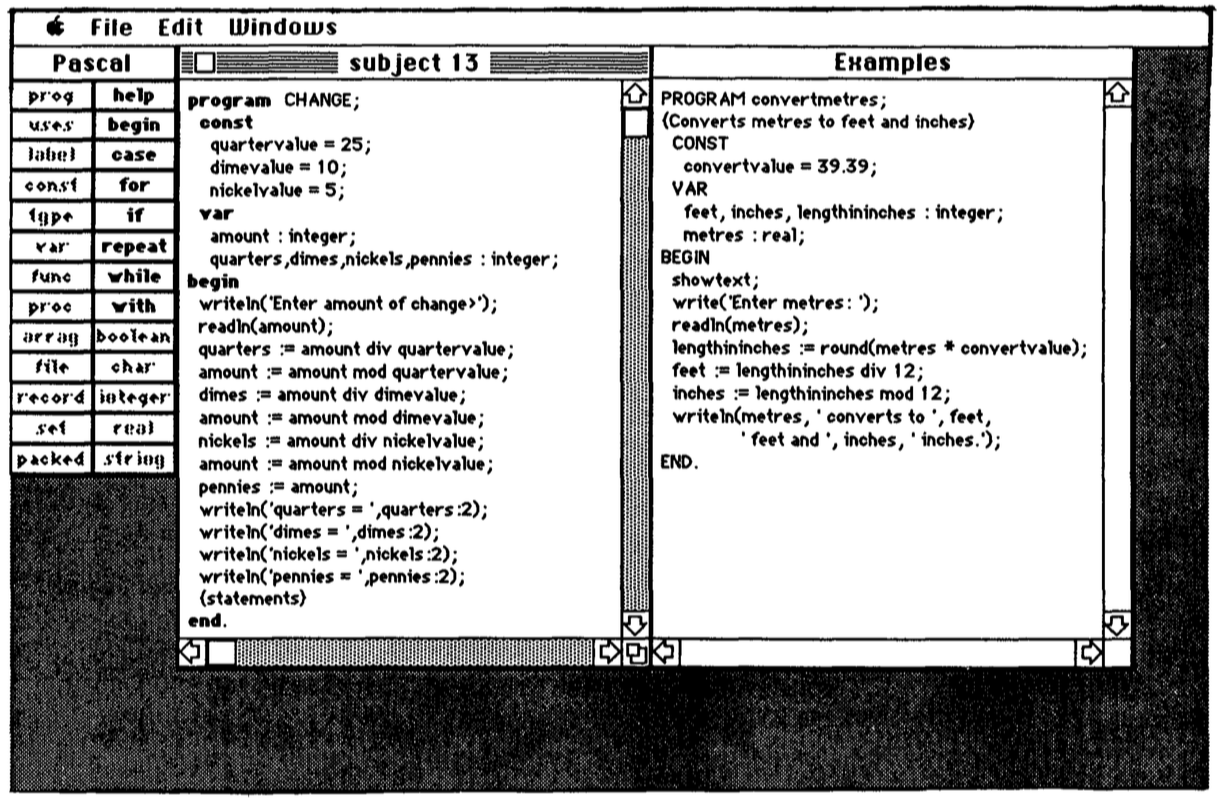
\includegraphics[width=0.95\textwidth]{Figures/tools/neal.png}
  \caption{Codeeditor mit Anwendungsbeispielen \citep{Neal:1989ef}}
  \label{fig:neal}
\end{figure}


Das Eclipse-Plugin \textit{eMoose}\footnote{\url{https://code.google.com/p/emoose-cmu/}} \cite{dekel2011increasing} verringert die Fehlerquote von API-Anwendern beim Gebrauch einer API. Dazu werden die im \sref{sec:api-directives} vorgestellten API-Direktiven im Editor eingeblendet (siehe \fref{fig:KnowledgePushing}). In der aktuellen Fassung des seit der Veröffentlichung nicht mehr aktualisierten Werkzeugs müssen die API-Direkten manuell von den API-Entwicklern beschrieben werden.

\begin{figure}
  \centering
    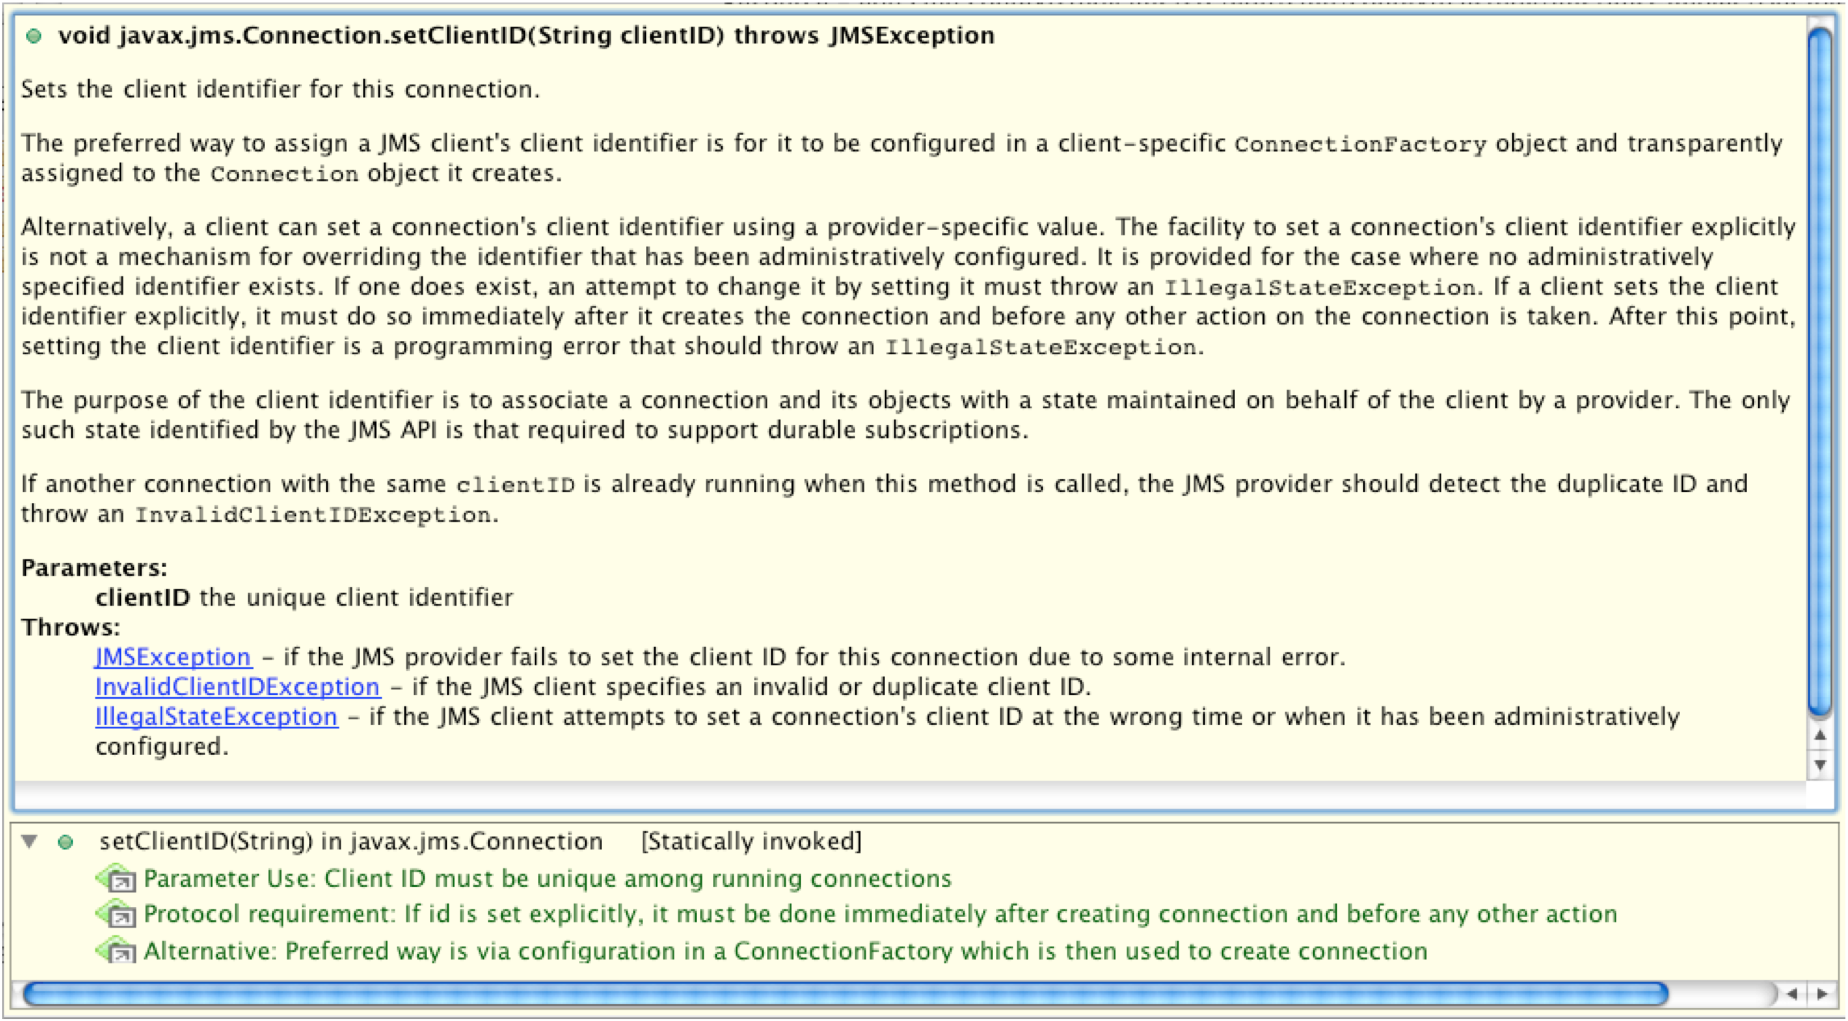
\includegraphics[width=0.8\textwidth]{Figures/tools/KnowledgePushing.png}
  \caption{Beispiel eines Eclipse-JavaDoc-Hilfdialogs für polymorphen Code \citep{dekel2011increasing}}
  \label{fig:KnowledgePushing}
\end{figure}


\textit{CodeBroker} \citep{Ye:2002fd} ist ein Emacs\footnote{\url{https://www.gnu.org/software/emacs/}}-Plugin, das den bereits vom API-Anwender geschriebenen Code mit einem \textit{reuse repository} abgleicht (siehe \fref{fig:CodeBroker}). Diese Informationen werden genutzt, um dem API-Anwender wichtige API-Informationen anzuzeigen, von denen das Werkzeug glaubt, dass sie dem API-Anwender unbekannt sind.

\begin{figure}[!ht]
  \centering
    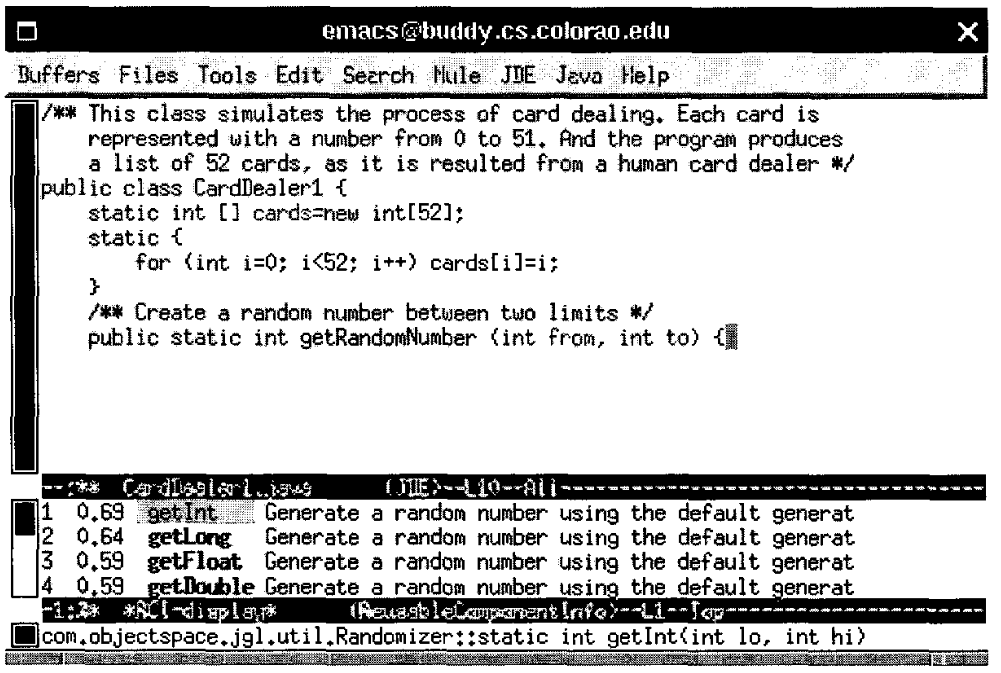
\includegraphics[width=0.75\textwidth]{Figures/tools/CodeBroker.png}
  \caption{CodeBroker \citep{Ye:2002fd}}
  \label{fig:CodeBroker}
\end{figure}


\textit{Better Code Completion (BCC)} \citep{Hou:2010fd} wurde als Erweiterung der Eclipse-Autovervollständigung entwickelt und verbessert sie wie folgt:
\begin{itemize}
  \item BCC unterscheidet zwischen dem \texttt{public}-Modifizierer und dem neu eingeführten \texttt{API-public}-Modifizierer.
  \item Methoden werden logisch nach Anwendungskontexten gruppiert.
  \item Codevervollständigungsvorschläge werden logisch und nach ihrer Popularität sortiert.
\end{itemize}
Das Werkzeug setzt Zuarbeiten durch die API-Entwickler voraus.


Das Werkzeug \textit{XFinder} \citep{Dagenais:2008kj} unterstützt API-Anwender ebenfalls durch das automatische Auffinden von Beispielen für konkrete Aufgaben. Im Gegensatz zum weiter oben vorgestellten \textit{Strathcona} benötigt dieses Werkzeug jedoch eine API-Dokumentation und damit die Zuarbeit von API-Entwicklern, um Beispiele aufzufinden. Dafür eignet sich das Werkzeug besser für Aufgaben, bei denen eine Vielzahl von Klassen gemeinsam verwendet werden müssen.


Das Eclipse-Plugin \textit{SnipMatch}\footnote{\url{http://snipmatch.com}} \citep{Wightman:2012gc} hat sich auf den Komfort von Codefragment-Einfügeoperation spezialisiert. So erlaubt es beispielsweise interaktiv, die im Codefragment verwendeten Bezeichner an die des Zielprogramms anzupassen. Als Datengrundlage dienen so genannte Snippets, die entweder von API-Entwicklern bereitgestellt oder von API-Anwendern selbst geschrieben werden müssen.


\textit{Mica}\label{sec:mica} \citep{Stylos:2006gu} ist ein prototypische Suchmaschinenerweiterung (siehe \fref{fig:mica}), die eine leichtere Auffindbarkeit von API-Klassen und -Methoden unter Zuhilfenahme der Google-Suchmaschine ermöglicht. Mica ordnet dabei die Ergebnisse abhängig von der Verwendungshäufigkeit der API-Klassen und -Methoden in Programmen. Des Weiteren werden Suchtreffer durch Anwendungsbeispiele angereichert. Zwar handelt es sich bei Mica nicht um ein Dokumentationssystem, nutzt letzteres aber indirekt intensiv.

\begin{figure}[ht!]
  \centering
    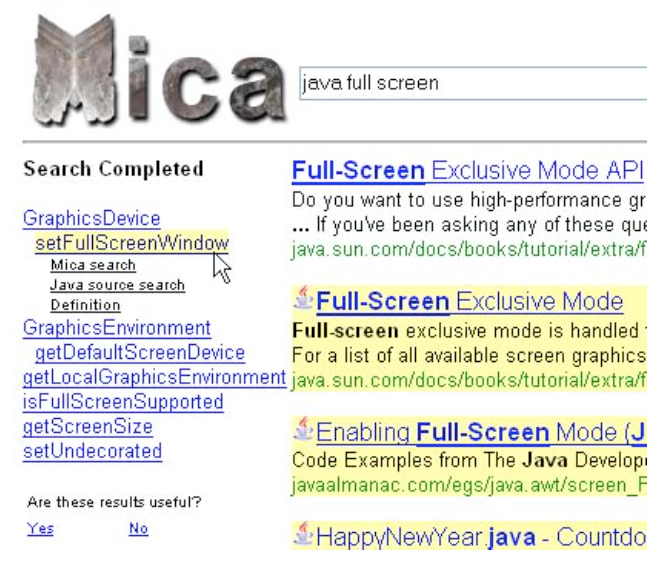
\includegraphics[width=0.6\textwidth]{Figures/tools/mica.png}
  \caption{Mica-Webapplikation \citep{Stylos:2006gu}}
  \label{fig:mica}
\end{figure}


\begin{important}
\textit{Jadeite}\label{sec:Jadeite}\footnote{\url{http://edelstein.pebbles.cs.cmu.edu/jadeite/}} \citep{Stylos:2009gc} ist ein an JavaDoc angelehntes Dokumentationssystem (siehe \fref{fig:jadeite}) und steht für ``\textbf{J}ava \textbf{A}PI \textbf{D}ocumentation with \textbf{E}xtra \textbf{I}nformation \textbf{T}acked-on for \textbf{E}mphasis''. Es basiert auf den Erkenntnissen vorangegangener Arbeiten \citep[insb. ][]{Furnas:1987hl,Stylos:2007jb,Stylos:2008jt} und verbessert JavaDoc durch die Unterstützung von Aliassen\footnote{Die Arbeit spricht von \textit{Platzhaltern}. Platzhalter kann es für Klassen und Methoden geben. Auf diese Weise erlauben die Autoren dem API-Anwender beispielsweise das Auffinden einer Methode, in einer anderen Anfangsklasse als der von den API-Entwicklern vorgesehenen Klasse.}, Konstruktionsbeispielen für Objekte und Hervorhebungen häufig genutzter Klassen und Methoden.
\end{important}

\begin{figure}[ht!]
  \centering
    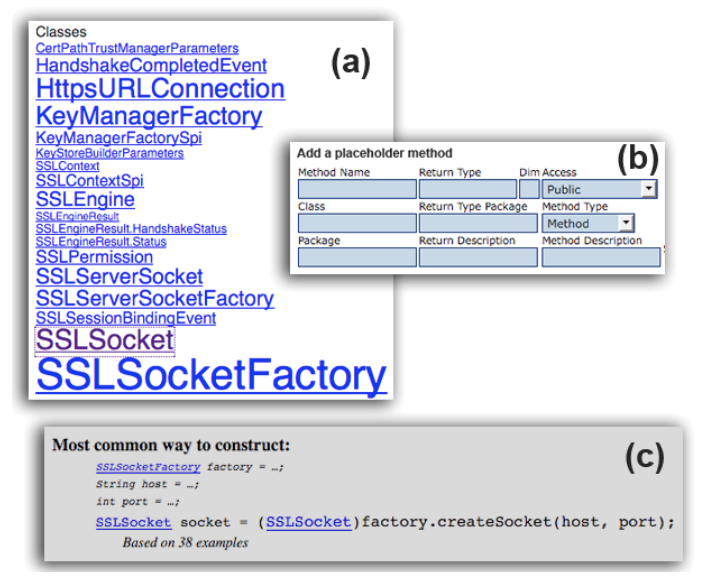
\includegraphics[width=0.75\textwidth]{Figures/tools/jadeite.png}
  \caption{Jadeite-Dokumentationssystem \citep{Stylos:2009gc}}
  \label{fig:jadeite}
\end{figure}


Das Werkzeug \textit{Apatite} \citep{Eisenberg:2010bm,Eisenberg:2010ds} ist ein Dokumentationssystem (siehe \fref{fig:apatite}), das API-Anwendern das Erlernen und Verstehen von komplexen \glslink{api}{APIs} erleichtern soll. Während in klassischen Dokumentationen eine hierarchische Gliederung anzutreffen ist, macht Apatite regen Gebrauch von Assoziationen zwischen den dokumentierten Elementen wie Klassen und Methoden. Den Einstieg in eine Apatite-basierte Dokumentation bildet eine Sucheingabe. Populäre Einträge werden dabei kontextabhängig hervorgehoben. Relationen berechnet das Werkzeug auf der Grundlage von Suchmaschinen und dem Quellcode der Softwarebibliothek.

\begin{figure}[!ht]
  \centering
    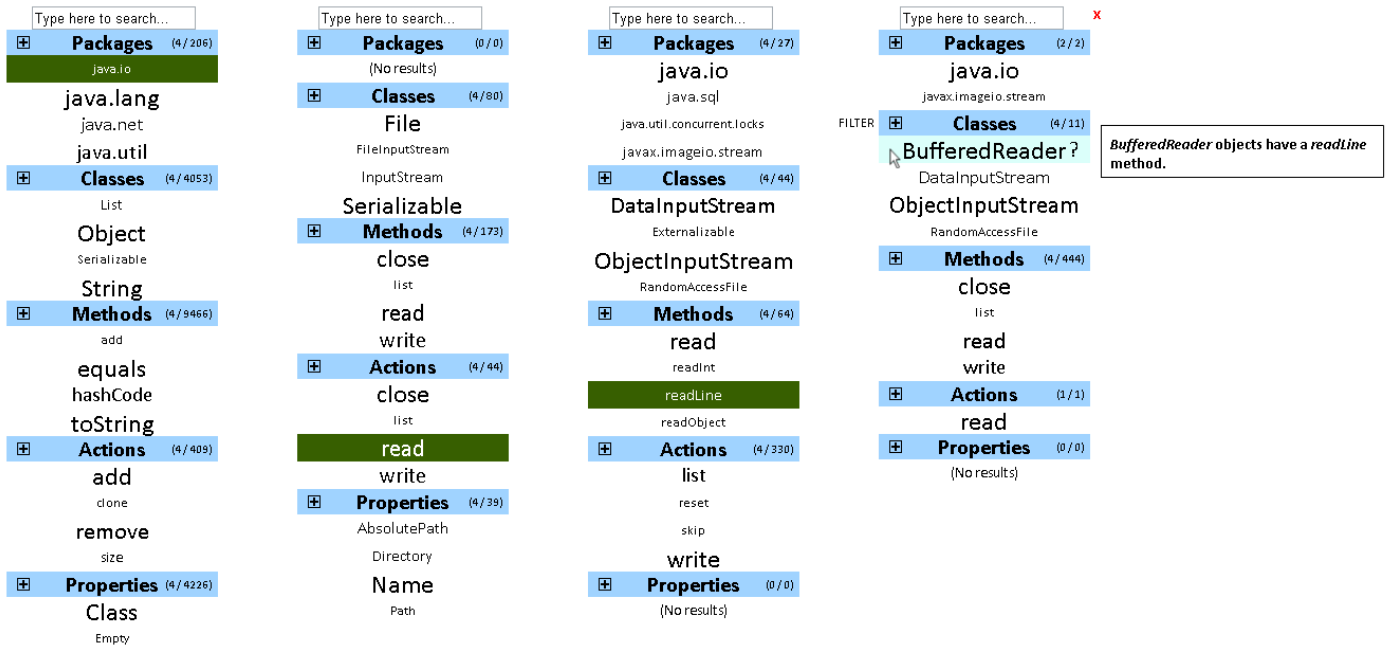
\includegraphics[width=1.0\textwidth]{Figures/tools/apatite.png}
  \caption{Apatite-Dokumentationssystem \citep{Eisenberg:2010bm}}
  \label{fig:apatite}
\end{figure}




\subsection{Werkzeuge für API-Anwender und -Endanwender}

Wie bereits im \sref{sec:euse} beschrieben, stellen API-Endanwender besondere Anforderungen an eine benutzerfreundliche \gls{api}. Die meisten hier vorgestellten Werkzeuge richten sich an API-Anwender, obwohl sie sich auch besonders gut für API-Endanwender eignen.

\begin{important}
Webforen\footnote{auch als Internet- oder Diskussionsforum bezeichnet} haben sich als nützliche Möglichkeit herausgestellt, eine andauernde Kommunikation zwischen API-Entwicklern und -Anwendern zu ermöglichen. Sie stellen eine exzellente Ressource für die Themen Debugging, Bugs und Entwurfsfragen dar. \citep{DaqingHou:2005ba}
\\Darüber hinaus bergen Webforen das Potential, API-Endanwendern das Wissen und die Hilfe von erfahrenen API-Anwendern zugänglich zu machen. \citep{Ko:2005cl}
\end{important}


Ein zu SnipMatch ähnlichen Ansatz verfolgen \cite{Oney:2012ge}. Sie führen den Begriff von \textit{Codelets} ein. Darunter verstehen sie semantisch abgeschlossene Stücke Beispielcode, die, nachdem sie in den Editor eingefügt wurden, auch später noch grafisch bearbeitet werden können. Indem eingefügter Code auch nach Programmierfortschritten vom Editor immer noch als Codelet-Instanzen erkannt werden (siehe \fref{fig:codelets}), eignen sie sich hervorragend für API-Endanwender. Jedoch müssen die Codelets zuvor von professionellen Entwicklern implementiert worden sein. Eine prototypische IDE-Integration wurde für den \textit{Ajax.org Cloud9 Editor}\footnote{\url{http://ace.c9.io}} entwickelt. 

\begin{figure}[!ht]
  \centering
    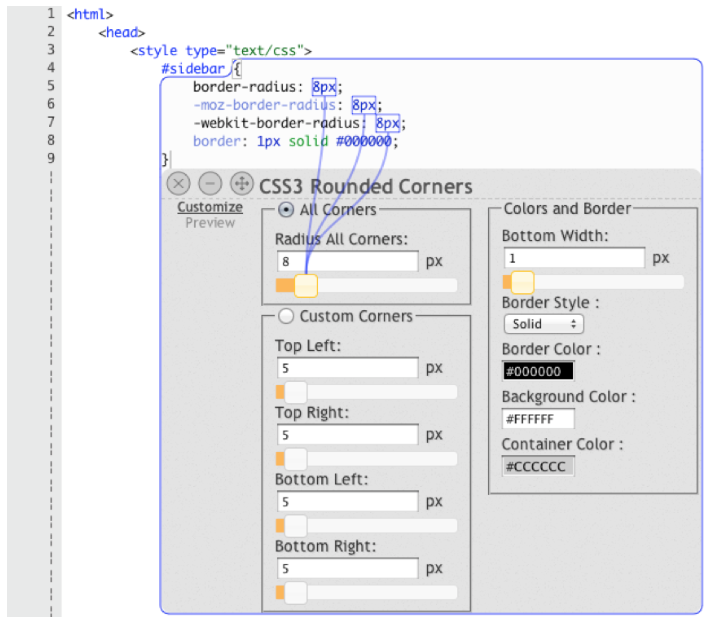
\includegraphics[width=0.75\textwidth]{Figures/tools/codelets.png}
  \caption{Codelets-Integration in Webeditor \citep{Oney:2012ge}}
  \label{fig:codelets}
\end{figure}


\textit{Graphite} \citep{Omar:2012tw} ist eine Erweiterung des Eclipse-Autovervollständigungsassistenten, die den Vervollständigungsdialog mit Hilfe von \textit{Paletten} ersetzt. Schreibt der API-Anwender beispielsweise \texttt{return} in einer Methode, die ein Objekt vom Typ \texttt{Color} zurückgibt, öffnet sich eine grafische Farbauswahl, die nach der Farbauswahl den korrekten Code für die Instanziierung der gewählten Farbe generiert.


\textit{Precise} \citep{Zhang:2012wl} ist ein Eclipse-Plugin, dass die Autovervollständigung erweitert. Im Gegensatz zu den anderen Lösungen vervollständigt dieses Werkzeug einzelne Methoden-Parameter (siehe \fref{fig:precise}).

\begin{figure}[!ht]
  \centering
    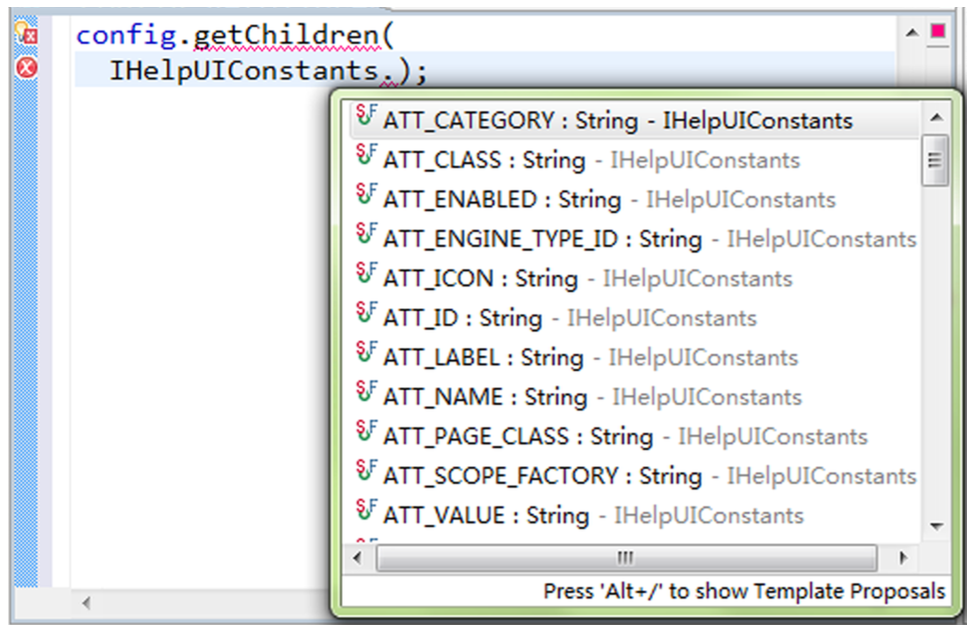
\includegraphics[width=0.55\textwidth]{Figures/tools/precise.png}
  \caption{Precise-Eclipse-Plugin \citep{Zhang:2012wl}}
  \label{fig:precise}
\end{figure}


\textit{EUKLAS} \citep[\textbf{E}clipse \textbf{U}sers’ \textbf{K}eystrokes \textbf{L}essened by \textbf{A}ttaching from \textbf{S}amples;][]{Doerner:2014cm} ist ein Eclipse-Plugin, das sich voll und ganz der Wiederverwendung von Beispielen verschrieben hat. Es ist behilflich bei typischen Probleme, die beim Einfügen von dritten Beispielcode auftreten. Leider ist die Erweiterung entgegen ihres generischen Namens auf die prototypische Programmiersprache JavaScript beschränkt.


\textit{Strathcona} \citep{Holmes:2005cm} ist ein Eclipse-Plugin, das es API-Anwendern ermöglicht, nach passenden Beispielcode zu suchen (siehe \fref{fig:strathcona1}) und zu übernehmen (siehe \fref{fig:strathcona2}). Neuartig an diesem Werkzeug ist, dass es den strukturellen Kontext für die Suche nutzt und die Code-Beispielen selbstständig heuristisch erzeugt.

\begin{figure}[!ht]
  \centering
    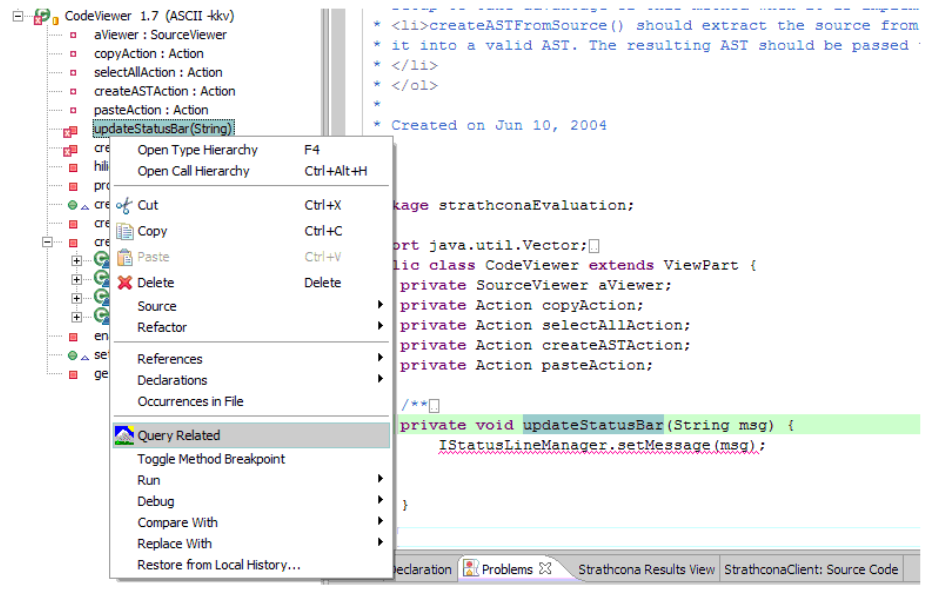
\includegraphics[width=0.85\textwidth]{Figures/tools/strathcona1.png}
  \caption{Strathcona: Formulierung einer Beispiel-Suchanfrage \citep{Holmes:2005cm}}
  \label{fig:strathcona1}
\end{figure}

\begin{figure}[!ht]
  \centering
    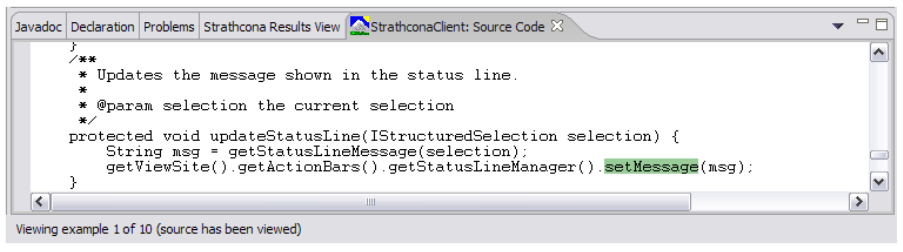
\includegraphics[width=0.75\textwidth]{Figures/tools/strathcona2.png}
  \caption{Strathcona: Einfügen des gewählten Beispielcodes \citep{Holmes:2005cm}}
  \label{fig:strathcona2}
\end{figure}


\textit{FrUit} \citep[\textbf{Fr}amework \textbf{U}nderstand\textbf{i}ng \textbf{T}ool integrated into Eclipse;][]{Bruch:2006bv} ist ein Eclipse-Plugin, das \textit{data-mining}-Techniken mit der von \cite{Holmes:2005cm} verwendeten Kontextsensitivität kombiniert (siehe \fref{fig:fruit}). Es unterstützt den Anwender dabei, typische API-Aufgaben zu lösen, indem es probabilistische Vorschläge für die nächsten Schritte unterbreitet. Dies zwingt den API-Anwender weit weniger, sich intensiv mit der API auseinandersetzen zu müssen, bevor er mit ihr arbeiten kann, was opportunistischen Entwicklern besonders entgegenkommt.

\begin{figure}[!ht]
  \centering
    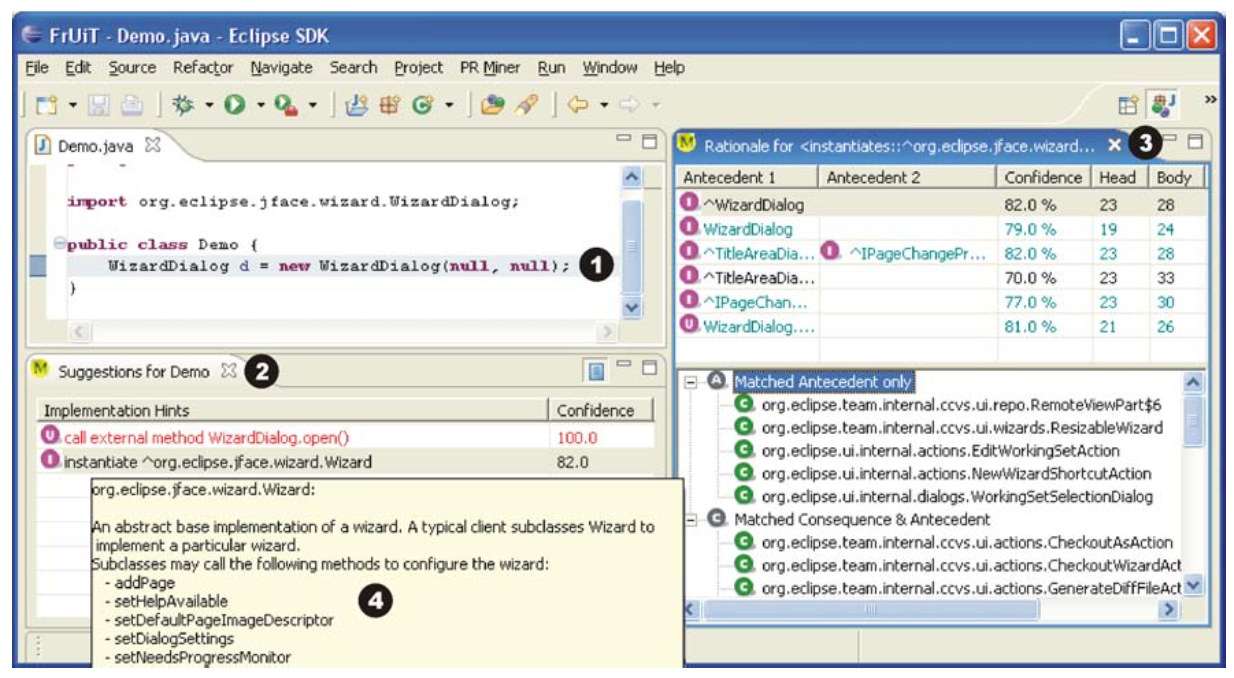
\includegraphics[width=0.9\textwidth]{Figures/tools/fruit.png}
  \caption{FrUit-Eclipse-Plugin \citep{Bruch:2006bv}}
  \label{fig:fruit}
\end{figure}


\textit{API Explorer} \citep{DualaEkoko:2011th} ist ein Eclipse-Plugin, dass sich primär der Auffindbarkeit relevanter API-Elemente wie Klassen und Methoden verschrieben hat. Während Jadeite \citep{Stylos:2009gc} ``nur'' Beispiele für die Erzeugung von Instanzen darstellt, kann API Explorer seine gemachten Vorschläge auch direkt in den Codeeditor einfügen (siehe \fref{fig:apiexplorer1}). Die zweite und wichtigere Funktion besteht darin, für eine Aufgabe relevante Klassen und Methoden zu finden und deren Anwendung ebenfalls direkt in den Codeeditor zu übernehmen (siehe \fref{fig:apiexplorer2}).

\begin{figure}[!ht]
  \centering
    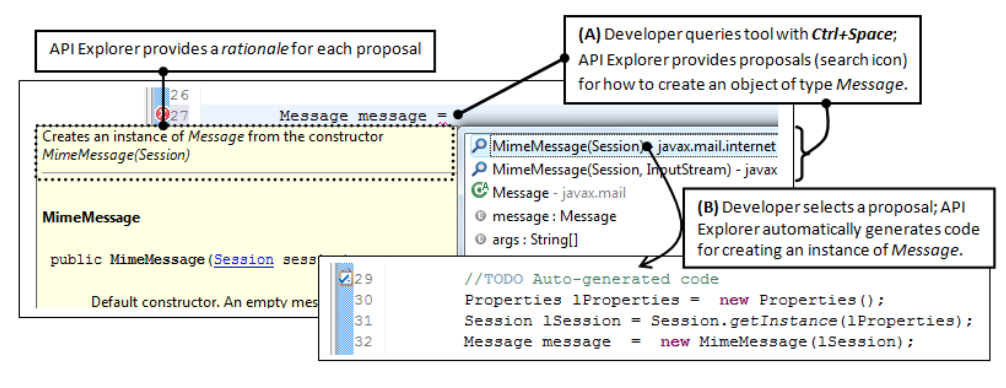
\includegraphics[width=1.0\textwidth]{Figures/tools/apiexplorer1.png}
  \caption{API-Explorer: Konstruktion einer Instanz \citep{DualaEkoko:2011th}}
  \label{fig:apiexplorer1}
\end{figure}

\begin{figure}[!ht]
  \centering
    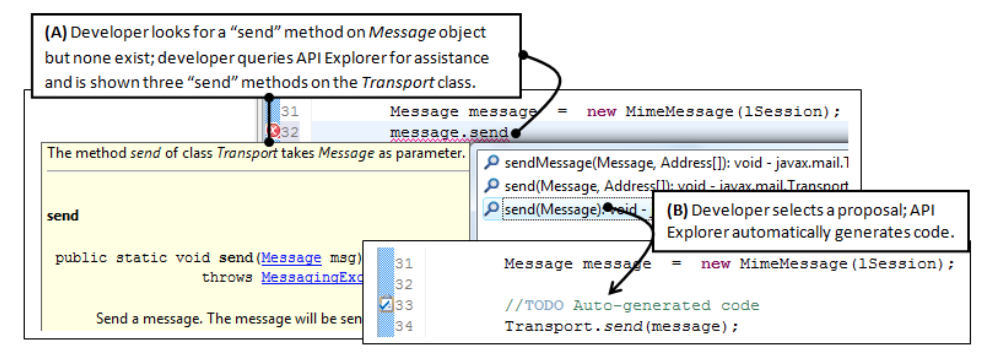
\includegraphics[width=0.95\textwidth]{Figures/tools/apiexplorer2.png}
  \caption{API-Explorer: Auffinden der zur \texttt{Message}-Klasse in Beziehung stehenden \texttt{Transport}-Klasse \citep{DualaEkoko:2011th}}
  \label{fig:apiexplorer2}
\end{figure}


\subsection{Werkzeuge ausschließlich für API-Endanwender}

Zwei Vertreter der Werkzeuge, die sich ausschließlich an API-Endanwender richten, nenne ich hier nur aus Gründen der Vollständigkeit und des Überblicks über die enorme Spannbreite an Hilfestellungen. \gls{euse} ist ein wichtiges Forschungsgebiet, das allerdings nicht im Fokus meiner Arbeit steht.

\textit{Whyline} \citep{Ko:2004fc} ist eine Debugger-Erweiterung für die Endanwender-Programmierer-Entwicklungsumgebung \textit{Alice}\footnote{\url{http://www.alice.org/index.php}}, die auf die --- ebenfalls in der Arbeit veröffentlichten, empirisch belegten --- Anforderungen dieser Anwendergruppe in Bezug auf Debugging eingeht. Die Forscher haben sich mit der Frage beschäftigt, wie ein Werkzeug Endanwender-Programmierer bei Beantwortung von Warum- und Warum-nicht-Fragen behilflich sein kann.

\begin{important}
Abschließend sei die Entwicklungsumgebung \textit{Dinah} \citep{Gross:2011ie} genannt. Für meine Forschung interessant sind die zugrunde liegenden Forschungsergebnisse. Sie zeigen, dass für Endanwender-Programmierer Beispiel-Code schätzen, aber mit dem \textit{Auswahl-Problem} konfrontiert sind \citep{Gross:2010hb}. Es besteht darin, dass (1) Endanwender häufig ihre Aufgabe zu abstrakt formulieren, um ein Beispiel zu finden, (2) der für die Lösung notwendige Code zu sehr verteilt ist, oder (3) die wichtigen von den weniger wichtigen Codezeilen des gefundenen Beispiels nicht unterschieden werden können.
\end{important}
\label{sec-end:forschungsstand}